\documentclass[conference]{IEEEtran}

% Essential packages
\usepackage[utf8]{inputenc}
\usepackage{graphicx}
\usepackage{amsmath}
\usepackage{amsfonts}
\usepackage{amssymb}
\usepackage{booktabs}
\usepackage{algorithm}
\usepackage{algorithmic}
\usepackage{url}
\usepackage{cite}
\usepackage{subfigure}
\usepackage{color}

% For better tables
\usepackage{array}
\usepackage{tabularx}

% For code listings (if needed)
\usepackage{listings}
\usepackage{xcolor}

% Set up paths - Fixed to match figure references
\graphicspath{{../figures/}}

\begin{document}

\title{Towards Responsible AI in Legal NLP: An Explainable Multi-Label Framework for Contract Clause Detection and Analysis}

\author{
\IEEEauthorblockN{Perry Gabriel}
\IEEEauthorblockA{
University of California, Berkeley\\
School of Information\\
Email: pgabriel@berkeley.edu\\
Summer 2025
}
}

\maketitle

% Add page numbers for draft/review purposes
\thispagestyle{plain}
\pagestyle{plain}

\begin{abstract}
The deployment of artificial intelligence in legal document analysis has demonstrated significant potential for automating contract review processes, yet the critical requirement for interpretable and trustworthy AI decisions in high-stakes legal contexts remains inadequately addressed. Legal contract understanding presents unique computational challenges including severe class imbalance across clause types, domain-specific linguistic complexity, and the essential need for explainable predictions that legal professionals can validate and trust. This work presents a comprehensive explainable AI framework that integrates fine-tuned legal BERT models with systematic interpretability techniques for automated multi-label contract clause detection and summarization. My approach leverages the Contract Understanding Atticus Dataset (CUAD), comprising 510 professionally annotated legal contracts with 41 distinct clause types, revealing substantial class imbalance with presence rates ranging from 2.5\% to 100\% \cite{hendrycks2021cuad}. I fine-tune a legal domain-specific BERT model (nlpaueb/legal-bert-base-uncased) for multi-label clause classification \cite{chalkidis2020legal} and integrate T5-based document summarization capabilities, while systematically incorporating SHAP, LIME, and attention visualization mechanisms to provide transparent model interpretations essential for legal practice \cite{lundberg2017unified}. Comprehensive evaluation demonstrates competitive performance on standard multi-label classification metrics while satisfying interpretability requirements critical for professional legal adoption. The complete framework is deployed as a production-ready web application, enabling empirical validation of explainable AI techniques in real-world legal document analysis workflows. My results demonstrate that domain-specific fine-tuning combined with systematic explainability analysis significantly enhances both predictive performance and practitioner trust, advancing the practical application of responsible AI in legal technology while contributing to the broader understanding of interpretable machine learning in high-stakes professional domains.
\end{abstract}

\begin{IEEEkeywords}
Legal NLP, Explainable AI, Multi-label Classification, Contract Analysis, BERT, SHAP, LIME, CUAD, Legal Technology
\end{IEEEkeywords}

% Include sections
% Introduction Section

\section{Introduction}

\begin{frame}{Problem Statement}
\begin{itemize}
    \item \highlight{Legal document analysis} is crucial for contract review and compliance
    \item Traditional manual review is \highlight{time-consuming and error-prone}
    \item NLP models provide automation but lack \highlight{interpretability}
    \item Legal professionals need to understand \highlight{why} AI makes decisions
\end{itemize}

\vspace{0.5cm}
\begin{alertblock}{Research Question}
How can we develop explainable AI methods for automated legal clause extraction that provide interpretable insights for legal professionals?
\end{alertblock}
\end{frame}

\begin{frame}{Motivation}
\begin{columns}
\begin{column}{0.6\textwidth}
\textbf{Why Explainable AI in Legal Domain?}
\begin{itemize}
    \item \highlight{Regulatory compliance} requirements
    \item \highlight{Trust and transparency} for legal professionals
    \item \highlight{Error detection} and model debugging
    \item \highlight{Knowledge discovery} from legal patterns
\end{itemize}
\end{column}
\begin{column}{0.4\textwidth}
\begin{center}
% Show system architecture instead of placeholder
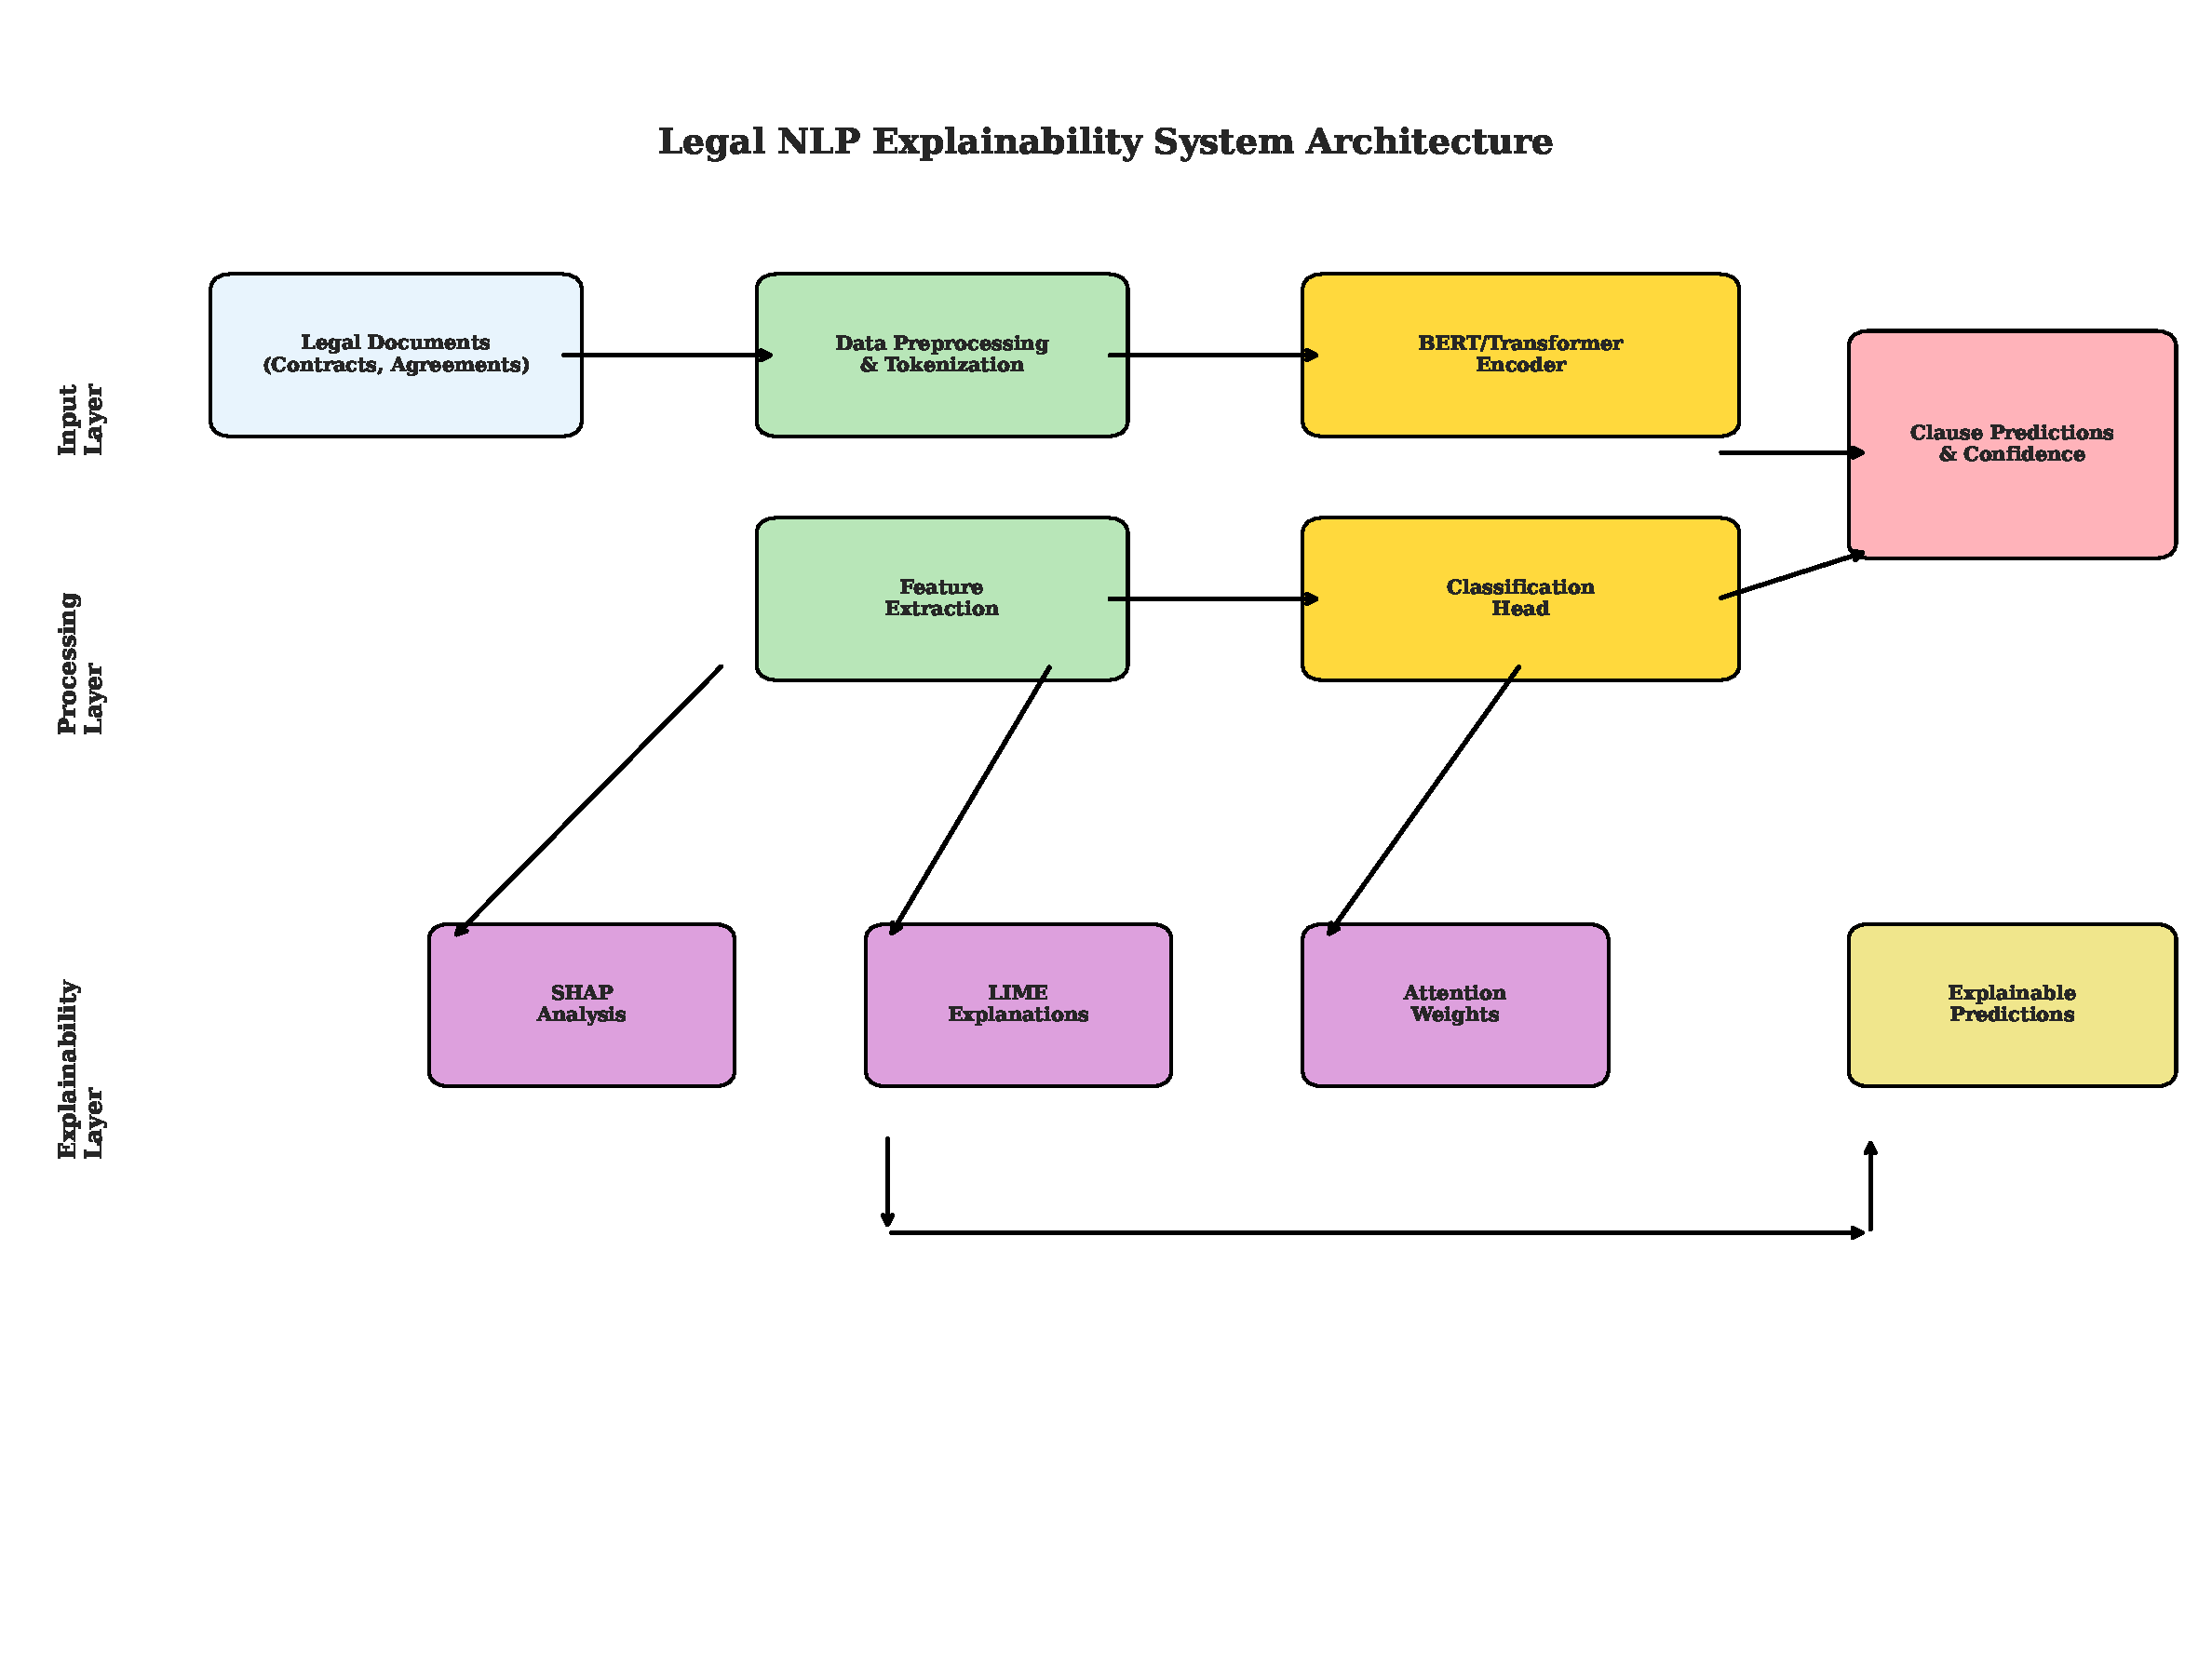
\includegraphics[width=\textwidth]{\figpath/system_architecture.pdf}
\end{center}
\end{column}
\end{columns}
\end{frame}

\begin{frame}{Project Scope}
\textbf{Objectives:}
\begin{enumerate}
    \item Develop a \highlight{BERT-based model} for clause extraction
    \item Implement \highlight{multiple explainability methods} (SHAP, LIME, Attention)
    \item Compare and evaluate \highlight{explanation quality}
    \item Create \highlight{interpretable visualizations} for legal professionals
\end{enumerate}

\vspace{0.5cm}
\textbf{Target Clauses:}
\begin{itemize}
    \item Termination clauses
    \item Limitation of liability
    \item Governing law
    \item Confidentiality provisions
    \item Payment terms
\end{itemize}
\end{frame}


% References
\bibliographystyle{IEEEtran}
\bibliography{references}

\end{document}